\documentclass[a4paper,8pt]{extarticle}\usepackage[]{graphicx}\usepackage[]{color}
%% maxwidth is the original width if it is less than linewidth
%% otherwise use linewidth (to make sure the graphics do not exceed the margin)
\makeatletter
\def\maxwidth{ %
  \ifdim\Gin@nat@width>\linewidth
    \linewidth
  \else
    \Gin@nat@width
  \fi
}
\makeatother

\definecolor{fgcolor}{rgb}{0.345, 0.345, 0.345}
\newcommand{\hlnum}[1]{\textcolor[rgb]{0.686,0.059,0.569}{#1}}%
\newcommand{\hlstr}[1]{\textcolor[rgb]{0.192,0.494,0.8}{#1}}%
\newcommand{\hlcom}[1]{\textcolor[rgb]{0.678,0.584,0.686}{\textit{#1}}}%
\newcommand{\hlopt}[1]{\textcolor[rgb]{0,0,0}{#1}}%
\newcommand{\hlstd}[1]{\textcolor[rgb]{0.345,0.345,0.345}{#1}}%
\newcommand{\hlkwa}[1]{\textcolor[rgb]{0.161,0.373,0.58}{\textbf{#1}}}%
\newcommand{\hlkwb}[1]{\textcolor[rgb]{0.69,0.353,0.396}{#1}}%
\newcommand{\hlkwc}[1]{\textcolor[rgb]{0.333,0.667,0.333}{#1}}%
\newcommand{\hlkwd}[1]{\textcolor[rgb]{0.737,0.353,0.396}{\textbf{#1}}}%
\let\hlipl\hlkwb

\usepackage{framed}
\makeatletter
\newenvironment{kframe}{%
 \def\at@end@of@kframe{}%
 \ifinner\ifhmode%
  \def\at@end@of@kframe{\end{minipage}}%
  \begin{minipage}{\columnwidth}%
 \fi\fi%
 \def\FrameCommand##1{\hskip\@totalleftmargin \hskip-\fboxsep
 \colorbox{shadecolor}{##1}\hskip-\fboxsep
     % There is no \\@totalrightmargin, so:
     \hskip-\linewidth \hskip-\@totalleftmargin \hskip\columnwidth}%
 \MakeFramed {\advance\hsize-\width
   \@totalleftmargin\z@ \linewidth\hsize
   \@setminipage}}%
 {\par\unskip\endMakeFramed%
 \at@end@of@kframe}
\makeatother

\definecolor{shadecolor}{rgb}{.97, .97, .97}
\definecolor{messagecolor}{rgb}{0, 0, 0}
\definecolor{warningcolor}{rgb}{1, 0, 1}
\definecolor{errorcolor}{rgb}{1, 0, 0}
\newenvironment{knitrout}{}{} % an empty environment to be redefined in TeX

\usepackage{alltt}
\usepackage[a4paper,top=3cm,bottom=2cm,left=2cm,right=2cm,marginparwidth=1.75cm]{geometry}
\usepackage[english]{babel}  % force American English hyphenation patterns
\usepackage[utf8]{inputenc}  % unicode
% \usepackage{graphicx}
% \usepackage{lipsum}  % generate text
\usepackage{xcolor}  % have more than basic colors
\definecolor{mygray}{rgb}{0.8,0.8,0.8}
\usepackage{hyperref}
%\usepackage{todo}
\usepackage{todonotes} % to be able to add corrections
\usepackage[color]{changebar}  % to be able to add corrections
\cbcolor{red} % color of the changebar
\usepackage[nottoc,notlot,notlof]{tocbibind} % makes bibliography appear in toc
\usepackage{listings}  % include code, code style
\lstset{basicstyle=\ttfamily, breaklines = true, backgroundcolor=\color{mygray},language=bash,basicstyle=\ttfamily,columns=fullflexible}
\usepackage{wrapfig}  % figures can be wrapped in text
\usepackage{mathtools}  % have math symbols
\usepackage{amsmath}
\usepackage{amssymb}
\usepackage{booktabs}  % to make professional tables
% ------------------------------------------------------------------------- document descriptions
\title{Signal and Image Processing - HW2}
\author{Noëlle Schenk}
\date{\today, time invested : 9.5h}
% ------------------------------------------------------------------------- literature references
\usepackage[backend=biber]{biblatex} % to use biber for my citations
\addbibresource{../../../literature/pc_exserta_reflist.bib} % where latex can find the .bib file
% -------------------------------------------------------------------------
\IfFileExists{upquote.sty}{\usepackage{upquote}}{}
\begin{document}
\maketitle
% \tableofcontents
% \newpage
\section{Comments}
Please note that I was not able to run the line \lstinline!from tools_template import *! and I don't know exactly why. As I think it will run on your system, I let this line in the code. However, the scripts also work if just \lstinline!python3 tools_template.py! followed by \lstinline!python3 <ex1-3>!, so I hope this counts as running code.

\section{Exercise 1}
Increasing filter size makes the dark border around the image to be thicker, as the code does handle borders by zero padding. If another way of handling borders would be chosen, this would change. Generally, a larger filter takes into account more neighbors and leads to a higher blurring intensity. \\
A large sigma gives more weight to far neighbors and therefore also leads to a higher blurring intensity.

\section{Exercise 2}
\begin{figure}
  \caption{Gaussian pyramid.}
  \centering
    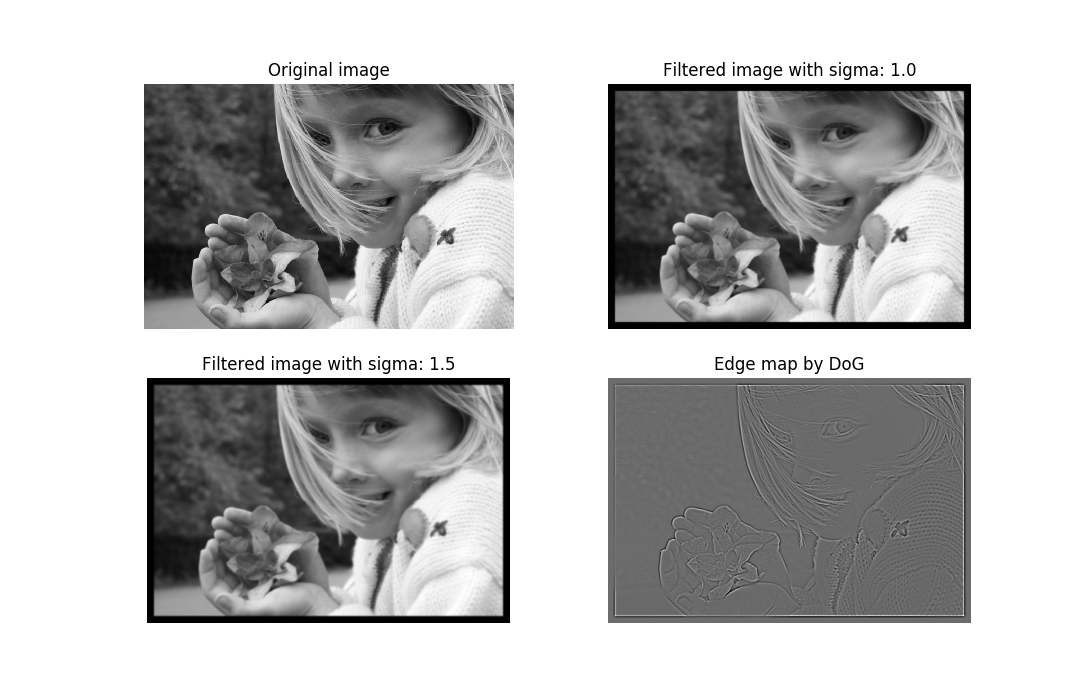
\includegraphics[width=0.49\textwidth]{figs/ex2_1.png}
    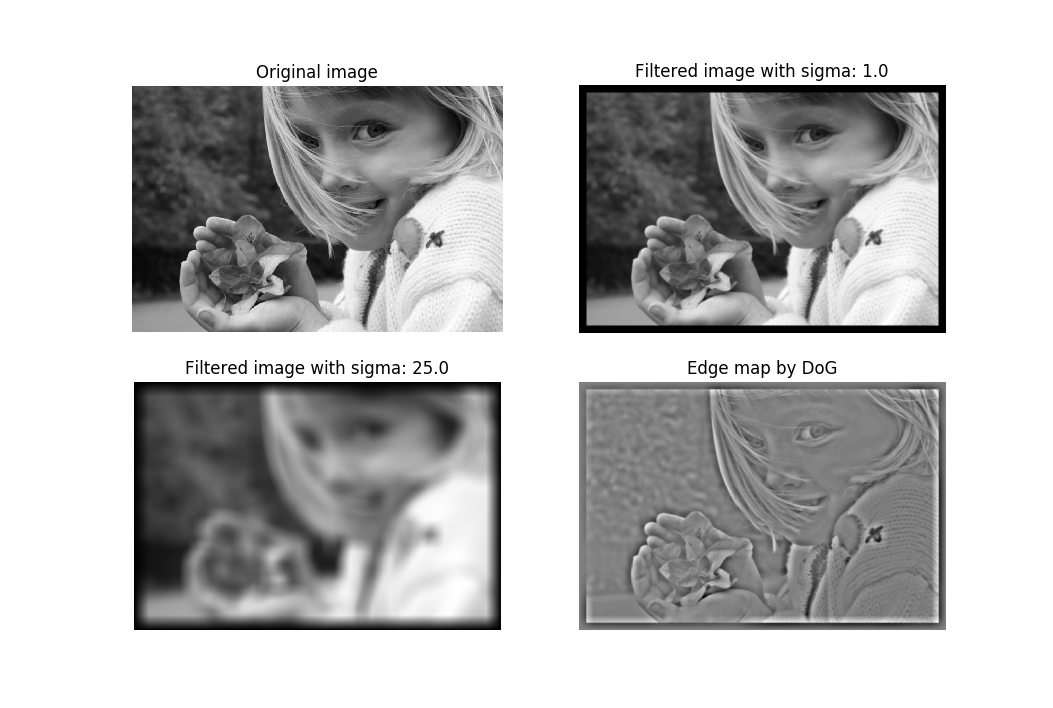
\includegraphics[width=0.49\textwidth]{figs/ex2_2.png}
  \label{fig:edges}
  \caption{Edge detection with different parameters. Left : $\sigma$ 1 = 1, $\sigma$ 2 = 1.5. Right : $\sigma$ 1 = 1, $\sigma$ 2 = 25, filter size 30 for both.}
\end{figure}

On Figure \ref{fig:edges} shows two edge detection outcomes with different parameters. The filter size was the same, only $\sigma$ 2 was changed. The difference in DoG are striking, on the left compared to the right, edges are much thinner and the whole image shows less standard deviation in grayscales (much less contrast). Probably, edges are detected better if the two sigma do not differ too much, not 25:1 as in the right image panel. \\
Smoothing removes small details and subtracting two smoothed images results in the DoG image that does not show small details any more, but traces the edges where pixel values change much. 

\section{Exercise 3.1 c}
\begin{figure}
  \caption{Gaussian pyramid.}
  \centering
    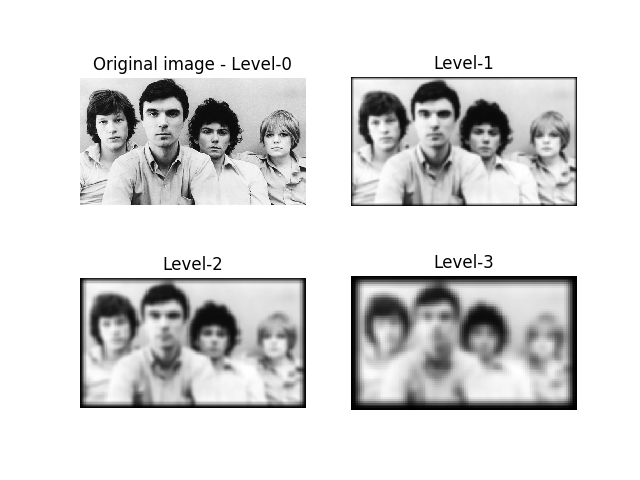
\includegraphics[width=0.6\textwidth]{figs/gaussian.png}
  \label{fig:gauss}
  \caption{Parameters : $\sigma$ = 4, scale = 0.6, filter size = 8, num levels = 4}
\end{figure}
The created gaussian pyramid can be seen in Figure \ref{fig:gauss}. 

\section{Exercise 3.4}
Increasing $\alpha$ from 0.56 to a higher value accepts less values to be "high". That means, less pixels are 1 and the face detection is more restrictive. If $\alpha$ is increased too much, probably only the best matching face is detected. \\
Decreasing $\alpha$ allows more pixels to reach a high score and therefore detects more faces. \\
Depending on the situation, either a very restrictive or the contrary can be of use, e.g. to identify face candidates which are later classfied by hand, it makes sense to allow many pixels to be identified as faces to capture all faces. If no classification by hand is done and it is not incredibly important to find all faces on a picture, a restrictive search (with a high $\alpha$) may fit better. \\
It is by the way also normal to not only detect the middle of the face (mostly the nose) at one given pixel but many pixels on the nose.

\section{Exercise 3.5}
\begin{figure}
  \caption{Gaussian pyramid.}
  \centering
    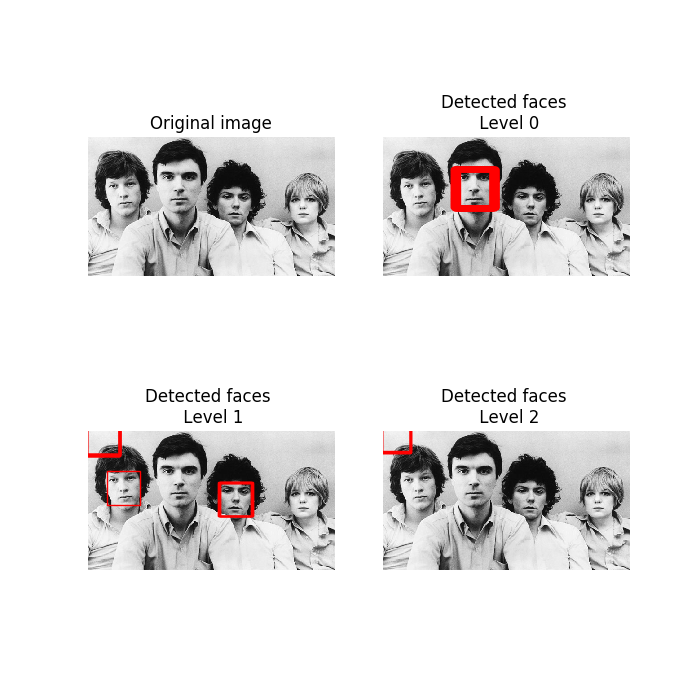
\includegraphics[width=0.6\textwidth]{figs/face_detection.png}
    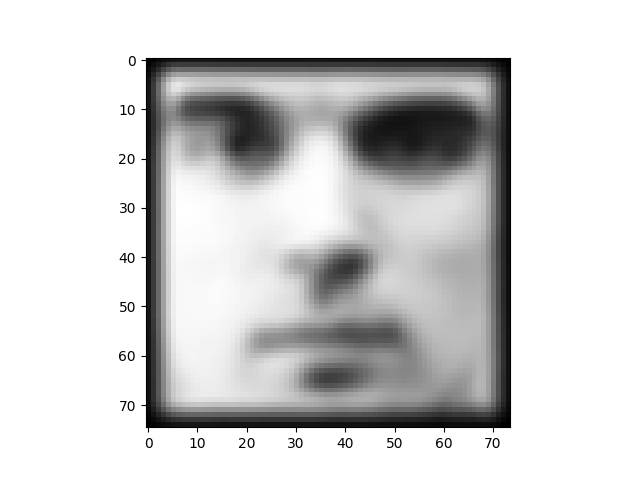
\includegraphics[width=0.1\textwidth]{figs/temp_level1.png}
  \label{fig:face}
  \caption{Detected faces (left) and the template which was used for level 1 (right).}
\end{figure}

Figure \ref{fig:face} shows the detected faces with the rectangles around them. It is interesting that at level 0, when the template is of original size, the face where the template is taken from is detected. The other faces don't match, as they do not fit the size. At level 1, the two smaller faces of men are detected, but also a rectangle at the upper left corner. The template used for level 1 detection is shown below in Figure \ref{fig:face}. Possibly, the dark borders match as well, however, this could easily be corrected by cutting away the dark corners or using another approach of dealing with the borders, e.g. Repetition or Reflection. \\
More possible pitfalls could be that only faces that look straight into the camera are detected. No faces from the side or from a given angle can be found. Further, only the faces that match a size of the gaussian pyramid can be detected. Then, only one template was used, which was the one detected at level 0. Of corse, this template matches best the same man. However, it would make sense at least using a template from a woman and a man, and if possible more templates. Further, this code only works for black and white images and I imagine that brighness also plays an important role. We only want to match the shapes, but what we do is also correlating the brightness which is useless in our case. \\ \\

Anyway, I think the most important are the sizes, if we only work with 3 levels of sizes, we can only detect roughly three levels of face sizes. With the implemented algorithm, it would be very easy to make more sizes and probably also detect the smallest face. \\
Further, the image could aso go through something like a brightness gaussian pyramid, so we would have different brighnesses of each template. Then, the dark borders need to be either cut away or omitted by another border approach. If we only want to detect faces from this image, we could aso take all faces as templates and test if the "right" match also shows the highest correlation (which was the case here). We don't have any smiling faces, so if we want to detect smiling faces or faces with other expressions, we need to include that also in our templates. 
I found it interesting that similarity between human does not play such a large role in this rough face detection, but more the general shape of a face. \\ \\

An alternative could be to work with edges, that means first detecting all edges in the original image and also the template and do the same face detection with these images. This would prevent the problems with brightness. However, in colored images the skin color could probably be an important indicator for a face. And some parts of the face are not really detectable by edges, e.g. the cheeks and depending on brightness also the chin. \\
Possibly, it could be an approach to separately detect eyes, noses, ears and other parts of faces and then overlap the individual correlations. We could identify a score to e.g. count in a given area how many face-parts matched and identify the most scoring areas. This would allow us to search for faces from the side as well. 


% cd ~/Documents/signal_and_image_processing/h2
% just run : ./runlatex.sh

% or run all following commands (are in runlatex.sh)
% KNITR
% pdflatex lab_knitr.tex
% pdflatex lab_knitr.tex
% biber lab_knitr
% pdflatex lab_knitr
% gnome-open lab_knitr.pdf
\end{document}
\grid
